\subsection{Fifteen tasks with instructions}
\label{sec:fifteen}

The five-task sequence was chosen by us. To see whether the picture holds on a sequence that we did
not choose, we ran the 15 tasks of the official order~1 of Super-NaturalInstructions, with the same
model, budget and code, for the certified switch and for the two published methods. It is one seed,
and each run took 3.1 to 3.5 hours on a free GPU.

\begin{table}[t]
  \caption{Fifteen-task sequence, original instructions (T5-base, 10 epochs per task, seed 42;
  re-test against all reference answers). Columns as in Table~\ref{tab:fivemain}; ``Changed'' counts
  test inputs of the first 14 tasks. One seed.}
  \label{tab:fifteenmain}
  \centering
  \small
  \setlength{\tabcolsep}{4pt}
  \begin{tabular}{lccccc}
    \toprule
    Method & \shortstack[c]{Score\\right after\\learning $\uparrow$} & \shortstack[c]{Final\\score $\uparrow$} & \shortstack[c]{Forgetting\\(points) $\downarrow$} & \shortstack[c]{Answers\\changed $\downarrow$} & Certified inputs \\
    \midrule
    \cert{} (ours) & 42.77 & 42.77 & 0.00 & 0 of 1{,}097 & 1{,}197 of 1{,}197 \\
    \nearest{} & 42.77 & 42.77 & 0.00 & 0 of 1{,}097 &  \\
    \centre{} & 42.77 & 42.63 & 0.15 & 2 of 1{,}097 &  \\
    \keyswitch{} & 42.77 & 42.77 & 0.00 & 0 of 1{,}097 &  \\
    \plain{} & 42.77 & 14.88 & 30.67 & 973 of 1{,}097 &  \\
    \midrule
    InfLoRA & 30.46 & 26.13 & 5.69 & 661 of 1{,}097 &  \\
    GainLoRA & 29.08 & 28.62 & 1.09 & 215 of 1{,}097 &  \\
    \bottomrule
\end{tabular}

\end{table}

\begin{figure}[t]
  \centering
  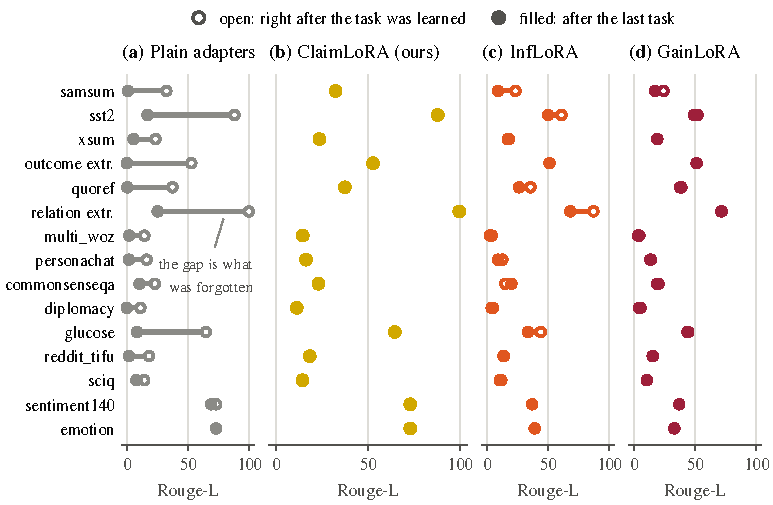
\includegraphics[width=\linewidth]{figures/fifteen_tasks}
  \caption{Score of each of the 15 tasks for four methods. Open circle: right after the task was
  learned. Filled circle: after the last task. A line between the two marks a change. For the
  certified switch the two circles coincide for every task.}
  \label{fig:fifteentasks}
\end{figure}

Table~\ref{tab:fifteenmain} and Figure~\ref{fig:fifteentasks} give the result. Appendix
Tables~\ref{tab:fifteenofficial} to \ref{tab:fifteenroutes} give the scores of the official script,
the scores for each wording, the scores of each task and the routes.

\paragraph{The certified switch keeps every answer.} The average score after the 15th task equals
the average score right after learning, \FifteenCertAP{} Rouge-L. Forgetting is \FifteenCertFT{},
and none of the \FifteenCertCompared{} answers to the test inputs of the first 14 tasks differs from
the answer given when the task had just been learned. All \FifteenCertInputsOne{} test inputs lie
inside their own zone, and no training input of a later task lay inside an older zone
(\FifteenCertBlocked{} of \FifteenCertTrainInputs{}). This is the outcome that Theorem~\ref{thm:writeonce}
guarantees. With the original instructions \nearest{} and \keyswitch{} give the same numbers, so
simpler rules reach the same score on this benchmark. \centre{} changes \FifteenCentreChanged{}
answers.

\paragraph{The same adapters without a switch lose most of what they learned.} With all adapters on,
the average falls from \FifteenPlainLearned{} to \FifteenPlainAP{}, forgetting is
\FifteenPlainFT{} points, and \FifteenPlainChanged{} of \FifteenPlainCompared{} answers change. The
score of every task except the last one falls (Table~\ref{tab:fifteenpertask} in the appendix).

\paragraph{The published methods learned less, and on fifteen tasks they also forget.} InfLoRA and
GainLoRA, run with their official code, end at \FifteenInfAP{} and \FifteenGainAP{}. On five tasks
neither forgot. Here InfLoRA forgets \FifteenInfFT{} points and GainLoRA \FifteenGainFT{}; the
answers that differ at the end are \FifteenInfChanged{} of \FifteenInfCompared{} for InfLoRA and
\FifteenGainChanged{} of \FifteenGainCompared{} for GainLoRA. The forgetting of InfLoRA is not
spread evenly. Relation extraction falls from \FifteenInfRelationLearned{} to
\FifteenInfRelationEnd{}, SST-2 from 61.0 to 50.0, summarisation of dialogues (SAMSum) from \FifteenInfSamsumLearned{} to
\FifteenInfSamsumEnd{} and Glucose from \FifteenInfGlucoseLearned{} to \FifteenInfGlucoseEnd{}. Both
methods also learned less right after each task: \FifteenInfLearned{} and \FifteenGainLearned{} on
average, against \FifteenCertLearned{} for plain adapters. So the gap of their final scores to the
certified switch has two parts, a gap in learning and a smaller gap from forgetting. We do not say
why they learned less. The caveats of the five-task runs apply: the budget is a tenth of the
published one, the model is smaller, and one step of their code was computed with a substitute
(Appendix~\ref{app:impl}). The official-script scores of InfLoRA are identical to those of an earlier run of the same method on Google Colab with the same seed, so for
this method the two platforms gave the same result (unlike the two five-task runs of seed 42, \fivefull{}).

\paragraph{The official script shows forgetting where no answer changed.} The official script gives
the certified switch an AP of \FifteenCertOffAP{} and a forgetting of \FifteenCertOffFT{}
(Table~\ref{tab:fifteenofficial}), although it changes no answer. This is evaluation noise, not
forgetting. The official script scores each answer against one reference answer, picked at random
on every load. The re-test, which scores every answer against all references, reproduces the
answers of the official test on \FifteenCertSame{} of \FifteenCertSameOf{} inputs for the certified
switch, \FifteenInfSame{} of \FifteenInfSameOf{} for InfLoRA and \FifteenGainSame{} of
\FifteenGainSameOf{} for GainLoRA, and it finds that none of the \FifteenCertCompared{} answers of
the certified switch changed. When the claim is that nothing changed, the answers have to be
compared and not the scores. The official scores of InfLoRA and GainLoRA lead to the same reading as
the re-test (AP \FifteenInfOffAP{} and \FifteenGainOffAP{}).

\begin{table}[t]
  \caption{Fifteen-task sequence with the original and with reworded instructions. The five tasks
  that have rewordings are those of the five-task sequence; they sit inside the 15-task sequence.
  AP is the average score of these five tasks after the last task, and ``Answers changed'' counts
  the test inputs of the first four of them (of 400); in the column ``original'' it counts those of the first 14 tasks (of 1{,}097). The adapters are those of Table~\ref{tab:fifteenmain};
  nothing is retrained. The column ``original'' is the whole sequence of 15 tasks.}
  \label{tab:fifteenwordings}
  \centering
  \small
  \setlength{\tabcolsep}{3.5pt}
  \begin{tabular}{lcccccccc}
    \toprule
    & \multicolumn{4}{c}{Final score $\uparrow$} & \multicolumn{4}{c}{Answers changed $\downarrow$} \\
    \cmidrule(lr){2-5} \cmidrule(lr){6-9}
    Method & original & light & medium & heavy & original & light & medium & heavy \\
    \midrule
    \cert{} (ours) & 42.8 & 80.7 & 80.2 & 76.0 & 0 & 0 & 0 & 0 \\
    \nearest{} & 42.8 & 80.7 & 80.2 & 76.0 & 0 & 0 & 0 & 0 \\
    \centre{} & 42.6 & 80.7 & 72.0 & 57.5 & 2 & 0 & 29 & 100 \\
    \keyswitch{} & 42.8 & 39.6 & 40.4 & 36.1 & 0 & 316 & 313 & 310 \\
    \plain{} & 14.9 & 39.6 & 40.4 & 36.1 & 973 & 316 & 313 & 310 \\
    \midrule
    InfLoRA & 26.1 & 51.6 & 44.7 & 32.6 & 661 & 257 & 272 & 270 \\
    GainLoRA & 28.6 & 51.1 & 47.1 & 37.0 & 215 & 69 & 85 & 109 \\
    \bottomrule
\end{tabular}

\end{table}

\paragraph{Reworded instructions inside the long sequence.} Table~\ref{tab:fifteenwordings} repeats
the five-task test inside the 15-task sequence. For the certified switch the number of changed
answers is zero in every wording. The average score of the five tasks is \FifteenCertAPLight{},
\FifteenCertAPMedium{} and \FifteenCertAPHeavy{} for the light, medium and heavy rewording. The
guarantee covers all \FifteenCertZoneOneLight{} inputs of the light rewording. For the medium and
the heavy rewording only \FifteenCertZoneOneMedium{} and \FifteenCertZoneOneHeavy{} of
\FifteenCertInputsOneMedium{} inputs are inside a zone, so the zero is again not guaranteed there.
\FifteenCertRightLight{}\%, \FifteenCertRightMedium{}\% and \FifteenCertRightHeavy{}\% of the inputs
are given to their own task. The exact key ends where plain adapters end (\FifteenPlainAPLight{},
\FifteenPlainAPMedium{}, \FifteenPlainAPHeavy{}). The nearest-centre rule \centre{} fails here: it gives \FifteenCentreRightMedium{}\% and
\FifteenCentreRightHeavy{}\% of the inputs with medium and heavy rewording to their own task, and
\FifteenCentreChangedMedium{} and \FifteenCentreChangedHeavy{} of \FifteenCentreComparedHeavy{}
answers change. InfLoRA forgets \FifteenInfFTLight{} points with the light rewording and
\FifteenInfFTHeavy{} with the heavy one on these five tasks, GainLoRA \FifteenGainFTLight{} and
\FifteenGainFTHeavy{} (Table~\ref{tab:fifteenmore} in the appendix). These rewordings are the
machine-written development set (Section~\ref{sec:protocol}); this run does not make
them an independent test.
